% !TEX root = ../main_lecture_notes.tex
\chapter{Security of blockchain systems}\label{chap:security}
The security evaluation of blockchain systems consists in calculating the probability of a successful attack on the blockchain. We will focus, in \cref{sec:double_spending}, on the double spending attack which is concern for \PoW powererd cryptocurrency like teh bitcoin one. Security is also at risk when the node have an incentive to deviate from the prescribed protocol. \cref{sec:blockwithholding} discusses the opportunity for miner of \PoW equipped blockchain to resort to blockwithholding strategy to optimize their revenue. 

\section{Double-spending in PoW}\label{sec:double_spending}
A double spending attack aims at generating a concurrent blockchain to replace the main one. Consider the following scenario
\begin{enumerate}
	\item Marie sends to John BTC$10$
	\item The transaction from Marie to John is recorded in the blockchain
	\item John is advised for $\alpha$ confirmation, that is for $\alpha-1$ block to be appended after the block where the Marie to John transaction is recorded
	\item Once $\alpha$ confirmations have been sent, John ships the good
	\item Meanwhile, Marie has started working on her own blockchain version where the Marie to John transaction is replaced by a Marie to Marie transaction
	\item At the shipment date the main blockchain is ahead by $z$ blocks 
	\item Marie's goal is then to work on her blockchain branch to catch up with the main branch. If she manages to to that then her branch will replace the public branch and she recovers her bitcoin. She can therefore spend these bitcoins again hence the name double spending.
\end{enumerate}
The race between the two competing branches of the blockchain is summarized on \cref{fig:dp_illustration}.
\begin{figure}[ht!]
\begin{center}
\begin{tikzpicture}[-, >=stealth', auto, semithick, node distance=1cm]
% \tikzstyle{block} = [rectangle, draw, fill=blue!20,
%     text width=5em, text centered, rounded corners]
\tikzstyle{block}=[rectangle, fill=black,draw=black,thick,text=black,scale=1.5]
\tikzstyle{block}=[rectangle, fill=white,draw=black,thick,text=black,scale=1.5]
\tikzstyle{confirmed block}=[rectangle, fill=white,draw=blue,thick,text=black,scale=1.5]
\tikzstyle{bad block}=[rectangle, fill=white,draw=red,thick,text=black,scale=1.5]
\node[block]    (1)                     {\tiny $\text{M}\rightarrow \text{J}$};
\node[block]    (2)[right of=1]                     {};
\node[block]    (3)[right of=2]                     {};
\node[block]    (4)[right of=3]                     {};
\node[confirmed block]    (5)[right of=4]                     {};

\node[bad block]    (6)[below of=1]         {\tiny $\text{M}\rightarrow \text{M}$};
\node[block]    (7)[right of=6]         {};
\node[block]    (8)[right of=7]         {};
\path
(1) edge[ left]     node{}     (2)
(2) edge[ left]     node{}     (3)
(3) edge[ left]     node{}     (4)
(4) edge[ left]     node{}     (5)
(6) edge[ left]     node{}     (7)
(7) edge[ left]     node{}     (8);

\end{tikzpicture}
\end{center}
\caption{Double spending race illustrated, here we have $\alpha = 4$ and $z = 2$}
\label{fig:dp_illustration}
\end{figure}
\subsection{Random walk model}\label{ssec:double_spending_rw}
We define a discrete time stochastic process $(R_n)_{n\geq0}$ equal to the difference in length between the public and the private branch of the blockchain. At each time step a block is found, it belongs to the main branch with probability $p$ to the other branch with probability $q=1-p$. The parameter $p$ represents the proportion of hashpower owned by the honest miners, while $q$ is that of the attacker. We have
$$
R_0 = z\text{, and  }R_n = z+Y_1+\ldots+ Y_n.
$$
The $Y_i$'s are \iid random variables such that 
$$
\mathbb{P}(Y=1) = p\in (0,1)\text{, and }\mathbb{P}(Y=-1) = 1-p=q,
$$ 
$(R_n)_{n\geq0}$ is therefore a random walk on $\mathbb{Z}$. We assume that $p>q$ so that the attacker does not hold more than half of the total hashpower. Define the double spending time as 
$$
{\tau_0} = \inf\{n>0\text{ ; }R_n = 0\}.
$$
Our goal is to study the distribution of this stopping time with respect to the filtration 
$$
\mathcal{F}_n = \sigma(Y_1,\ldots, Y_n),\text{ }n\geq1.
$$ 
An illustration of this first-hitting time problem is provided in \cref{fig:double_spending_time}.
\begin{figure}[ht!]
\begin{center}
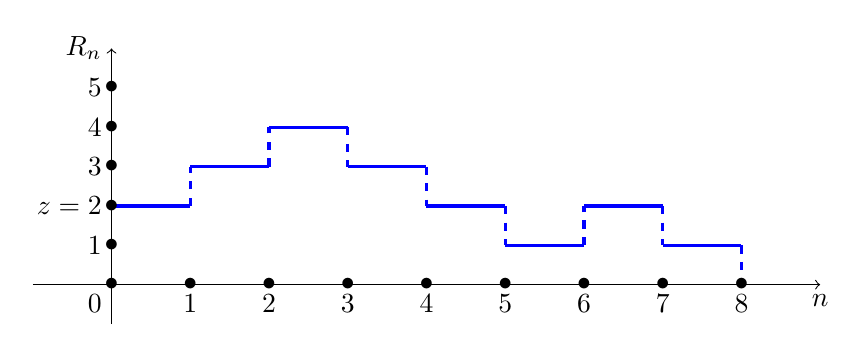
\begin{tikzpicture}
  %Origin and axis
  \coordinate (O) at (0,0);
  \draw[->] (-1,0) -- (9,0) coordinate[label = {below:$n$}] (xmax);
  \draw[->] (0,-0.5) -- (0,3) coordinate[label = {left:$R_n$}] (ymax);
  %Lower linear boundary

 
  %Stochastic process trajectory
  
  \draw (0,0) node[blue,left] {} node{};
  \draw[very thick,blue,-] (0,1) -- (1,1) node[pos=0.5, above] {} ;
  \draw[very thick,dashed,blue] (1,1) -- (1,1.5) node[pos=0.5, right] {};
  \draw[very thick,blue,-] (1,1.5) -- (2,1.5) node[pos=0.5, above] {};
  \draw[very thick,dashed,blue] (2,1.5) -- (2,2) node[pos=0.5, right] {};
  \draw[very thick,blue,-] (2,2) -- (3,2) node[pos=0.5, above] {};
  \draw[very thick,dashed,blue] (3,2) -- (3,1.5) node[pos=0.5, right] {};
  \draw[very thick,blue,-] (3,1.5) -- (4,1.5)node[pos=0.5, above] {};
  \draw[very thick,dashed,blue] (4,1.5) -- (4,1) node[pos=0.5, right] {};  
  \draw[very thick,blue,-] (4,1) -- (5,1) node[pos=0.5, above] {};
  \draw[very thick,dashed,blue] (5,1) -- (5,0.5) node[pos=0.5, right] {};  
  \draw[very thick,blue,-] (5,0.5) -- (6,0.5) node[pos=0.5, above] {};
  \draw[very thick,dashed,blue,-] (6,0.5) -- (6,1) node[pos=0.5, above] {};
   \draw[very thick,blue,-] (6,1) -- (7,1) node[pos=0.5, above] {};
    \draw[very thick,dashed,blue,-] (7,1) -- (7,0.5) node[pos=0.5, above] {};
     \draw[very thick,blue,-] (7,0.5) -- (8,0.5) node[pos=0.5, above] {};
     \draw[very thick,dashed,blue,-] (8,0.5) -- (8,0) node[pos=0.5, above] {};
  %Jump Times
  \draw (1,0) node[black,below] {$1$} node{ \color{black}$\bullet$};
  \draw (2,0) node[black,below] {$2$} node{ \color{black}$\bullet$};
  \draw (3,0) node[black,below] {$3$} node{ \color{black}$\bullet$};
  \draw (4,0) node[black,below] {$4$} node{ \color{black}$\bullet$};
  \draw (5,0) node[black,below] {$5$} node{ \color{black}$\bullet$};
  \draw (6,0) node[black,below] {$6$} node{ \color{black}$\bullet$};
  \draw (7,0) node[black,below] {$7$} node{ \color{black}$\bullet$};
  \draw (8,0) node[black,below] {$8$} node{ \color{black}$\bullet$};
  %Level of the counting process
   \draw (0,0) node[black,below left] {$0$} node{ \color{black}$\bullet$};
   \draw (0,0.5) node[black,left] {$1$} node{ \color{black}$\bullet$};
   \draw (0,1) node[black,left] {$z=2$} node{ \color{black}$\bullet$};
   \draw (0,1.5) node[black,left] {$3$} node{ \color{black}$\bullet$};
   \draw (0,2) node[black,left] {$4$} node{ \color{black}$\bullet$};
   \draw (0,2.5) node[black,left] {$5$} node{ \color{black}$\bullet$};

  % %Aggregated Capital gains
%  \draw (0,1.5) node[blue,below right] {$\mu_1$} node{ \color{blue}$-$};
%  \draw (0,2.25) node[blue,left] {$\mu_2$} node{ \color{blue}$-$};
%  \draw (0,3.75) node[blue,left] {$\mu_3$} node{ \color{blue}$-$};
  %Ruin time = First-crossing time time
%  \draw (5,0) node[black,above right] {${\tau_0}_u$} node{ \color{black}$\times$};
%  \draw[dotted,black] (0,3.28) -- (5,3.28);
%  \draw[dotted,black] (5,0) -- (5,3.28);
\end{tikzpicture}
\end{center}
\caption{Illustration of the first-hitting time problem of a double spending attack.}
\label{fig:double_spending_time}
\end{figure}
Let us denote by 
$$
\mathbb{P}_z(\cdot) = \mathbb{P}(\cdot|R_0 = z)\text{ and }\mathbb{E}_z(\cdot) = \mathbb{E}(\cdot|R_0 = z) 
$$
We are interested for now in the conditional distribution of ${\tau_0}$ provided that $R_0 = z$.
\subsubsection{Double spending probability}\label{sssec:double_spending_rw_dsp}
The double spending probability is defined as 
$$
\phi(z)=\mathbb{P}_z({\tau_0} <\infty),
$$
and given in the following result
\begin{theo}
If $p>q$ then 
$$
\phi(z) = \left(\frac{q}{p}\right)^z.
$$
\end{theo}
\noindent We give two proofs for this result, the first one uses simple first step analysis exploiting the Markov property of the random walk. The second one uses Martingale and the optional stopping theorem.\\

\underline{\textit Proof 1:}\\
Using a first step analysis, we have 
\begin{equation}\label{eq:difference_equation}
\phi(z) = p\phi(z+1)+(1-p)\phi(z-1),\text{ }z\geq1.
\end{equation}
We also have the boundary conditions
\begin{equation}\label{eq:boundary_conditions_double_spending}
\phi(0) = 1\text{ and }\underset{z\rightarrow +\infty}{\lim}\phi(z) = 0
\end{equation}
Equation \eqref{eq:difference_equation} is a linear difference equation of order $2$ associated to the following characteristic equation
$$
px^2 - x + 1-p = 0
$$
which has two roots on the real line with 
$$
r_1 = 1, \text{ and }r_2 = \frac{1-p}{p}.
$$
The solution of \eqref{eq:difference_equation} is given by 
$$
\phi(z)=A+B\left(\frac{1-p}{p}\right)^z,
$$
where $A$ and $B$ are constant. Using the boudary conditions \eqref{eq:boundary_conditions_double_spending}, we deduce that
$$
\phi(z) = \left(\frac{1-p}{p}\right)^z
$$
as announced.\\
For the second proof we need the notion of martingale
\begin{definition}
A stochastic process $(X_n)_{n\geq0}$, is called a martingale with respect to a filtration $\mathcal{F}_n$, if
\begin{itemize}
  \item[(i)] $X_n$ is $\mathcal{F}_n$-adapted
  \item[(ii)] $\mathbb{E}(X_n)<\infty\text{ for }n\geq\geq0$ 
  \item[(iii)] $\mathbb{E}(X_n|\mathcal{F}_{n-1}) = X_{n-1}$
\end{itemize} 
\end{definition}
\noindent and the optional stopping theorem.
\begin{theo}
Let $T$ be a stopping time for the Martingale $(X_n)_{n\geq0}$ then it holds that 
$$
\mathbb{E}(X_T) = \mathbb{E}(X_0) 
$$
in each of the following situations
\begin{itemize}
\item[(i)] $T$ is bounded almost surely 
\item[(ii)] There exists $c>0$ such that $|X_{T\land n}|<c$ for every $n>0$.
\item[(iii)] $\mathbb{E}(T)<\infty$, and, for some $K>0$ we have that 
$$
|X_n(\omega) - X_{n-1}(\omega)|\leq K,\text{ }\forall (n,\omega).
$$
\end{itemize}

\end{theo}
\underline{\textit Proof 2:}\\
Define the process 
$$
X_n = \exp\left[sR_n- n\kappa_Y(s)\right],\text{ for }n\in\mathbb{N}\text{ and }s\in\mathbb{R}, 
$$
where
$$
\kappa_Y(s) = \log\left[\mathbb{E}\left(e^{sY}\right)\right],
$$
is the cumulant generating function of $Y$. 
\begin{lemma}\label{lem:wald_martingale_RW}
Take $s$ so that $\kappa_Y(s)<\infty$ then $(X_n)_{n\geq0}$ is a $\mathcal{F}_n$-martingale.
\end{lemma}
\begin{proof}
Denote by $M_Y(s) = \mathbb{E}(e^{sY})$ the moment generating function of $Y$, we have that 
\begin{eqnarray*}
\mathbb{E}(X_n|\mathcal{F}_n)&=&\mathbb{E}\left\{\exp\left[sR_n - n\kappa_Y(s)\right]|\mathcal{F}_n\right\}\\
&=&\exp\left[sR_{n-1} - n\kappa_Y(s)\right]\mathbb{E}\left[\exp\left(sY_{n}\right)|\mathcal{F}_n\right]\\
&=&\exp\left[sR_{n-1} \right]M_Y(s)^{-n} M_Y(s)\\
&=& X_{n-1}.
\end{eqnarray*}
\end{proof} 
The equation $\kappa_Y(s) = 0$ is equivalent to 
$$
pe^s+qe^{-s} = 1
$$
which admits $\gamma =\log(q/p)$ as only non-zero solution. The process $(\e^{\gamma R_n})_{n\geq0}$ is a $\mathcal{F}_n$-Martingale. Define $\tau_a = \inf\{n\geq 0\text{ ; }R_n = a\}$, for $a>z$. Consider the stopping time $\tau = \tau_0\land\tau_a$, we have that for any $n>0$, 
$$
\mathbb{P}( \tau=\infty) \leq \mathbb{P}( \tau > n) < \mathbb{P}( |R_n| \leq a) \underset{n\rightarrow \infty}{\longrightarrow} 0;
$$
We can therefore apply the optional stopping time theorem at $\tau$ to get
\begin{eqnarray*}
 \mathbb{E}(X_{\tau}) = \mathbb{E}(X_{0})&\Leftrightarrow& \mathbb{P}(\tau = \tau_0) + [1- \mathbb{P}(\tau = \tau_0)]\e^{a z}= \e^{\gamma z}\\
 &\Leftrightarrow& \mathbb{P}(\tau = \tau_0)] = \frac{\e^{\gamma z}-\e^{a z}}{1-\e^{az}}.
\end{eqnarray*}
We then let $a\rightarrow\infty$ in the above equation to conclude that 
$$
\mathbb{P}(\tau = \tau_0) =\left(\frac{q}{p}\right)^z.
$$
\begin{exercise}
Just for fun
\begin{itemize}
\item What is $\phi(z)$ when $p \leq q$ ? 
\item Compute $\mathbb{P}(\tau_0 \leq \tau_a)$ if $p = q = 1/2$
\end{itemize}
\end{exercise}
In practice the number of blocks $z$ is actually random variable 
$$
Z = (\alpha -M)_+,
$$ 
where $M$ corresponds to the number of blocks the attacker managed to mine while the vendor waits for $\alpha$ confirmations. If we assume that a block mined by the honest miners is a success while a block mined by the attacker is a failure then $M$ actually counts the number of failure before $\alpha$ successes. We have that $M\sim \text{Neg-Bin}(\alpha, p)$ where $M$ has a probability mass function (\pmf) given by 
$$
\mathbb{P}(M = m) = \binom{\alpha+m-1}{m}p^\alpha q^m.
$$
Whenever $Z = 0$ then double spending occur right away as $\phi(0) =1$. To derive the double spending probability, we condition upon the values of $Z$ via the law of total probability 
$$
\mathbb{P}( \text{Double Spending}) = \mathbb{P}(M\geq \alpha)+\sum_{m = 0}^{\alpha-1}\binom{\alpha+m-1}{m}q^\alpha p^m.
$$
The analysis conducted here is similar to that of \citet{rosenfeld2014analysis}.
\subsubsection{Double spending time}\label{sssec:double_spending_rw_dst}
In the block mining world time is money. Every hour spent in computing hashes is costly in terms of energy. It is then very interesting to know whether a double spending attack is meant to last long or not. Intuitively, we can think that if it must occur the it should at a earlier stage because as $p>1/2$ our random walk $(R_n)_{n\geq0}$ will eventually drift toward $+\infty$. The following result provides the probability distribution of $\tau_0$ when $R_0 = z$.
\begin{theo}
If $z = 0$ then $\tau_0=0$ almost surely. If $z>0$ then $\tau_0$ admits a \pmf given by 
$$
\mathbb{P}_z(\tau_0 = n)=
\frac{z}{n}\binom{n}{(n-z) / 2}p^{(n-z) / 2}q^{(n
+z) / 2}\text{ if }n>z\text{ and }n-z\text{ is even},
$$
and $0$ otherwise.
\end{theo}
\begin{proof}
We start by showing the following lemma, sometimes referred to as the Markov hitting time theorem.
\begin{lemma}\label{lem:markov_hitting_time}
\begin{equation}\label{eq:markov_hitting_time}
\mathbb{P}_z(\tau_0 = n) = \frac{z}{n}\mathbb{P}_z(R_n = 0)
\end{equation}
\end{lemma}
\begin{proof}
If $z = 0$ then $\tau_0 = 0$ almost surely and both sides of \eqref{eq:markov_hitting_time} equal to $0$. Assume that $z\geq1$, we have that $\mathbb{P}_z(\tau_0 = n) = 0$ and $\mathbb{P}_z(R_n = 0) = 0$ whenever $n<z$ and $n-z$ is odd. The rest of the proof is by induction on $n\geq1$, when $n = 1$ we have that 
$$
\mathbb{P}_z(\tau_0 = 1) = 0 = \frac{z}{1}\mathbb{P}_z(R_1 = 0),\text{ for }z>1, 
$$
and 
$$\mathbb{P}_1(\tau_0 = 1) = q = \frac{1}{1}\mathbb{P}_1(R_1 = 0),\text{ for }z=1. 
$$
The property holds for $n=1$. Assume that it holds for some $n\geq1$. The law of total probability yields
\begin{eqnarray*}
\mathbb{P}_z(\tau_0 = n+1)&=&\sum_{y\in\{-1,1\}}\mathbb{P}_z(\tau_0 = n+1|Y_1 = y)\mathbb{P}(Y_1 = y)\\
&=&\sum_{y\in\{-1,1\}}\mathbb{P}_{z+y}(\tau_0 = n)\mathbb{P}(Y_1 = y)\\
&=&\sum_{y\in\{-1,1\}}\frac{z+y}{n}\mathbb{P}_{z+y}(R_n = 0)\mathbb{P}(Y_1 = y)
\end{eqnarray*}
The second equality holds thanks to the strong Markov property. We further undo the law of total probability.
\begin{eqnarray}
\mathbb{P}_z(\tau_0 = n+1)&=&\sum_{y\in\{-1,1\}}\frac{z+y}{n}\mathbb{P}_{z}(Y_1 = y|R_{n+1} = 0)\mathbb{P}_z(R_{n+1} = 0)\nonumber\\
&=&\frac{\mathbb{P}_z(R_{n+1} = 0)}{n}\left[z+\mathbb{E}(Y_1|R_{n+1}=0)\right]\label{eq:law_total_probability_undone}
\end{eqnarray}
Since the $Y_i$ are \iid then it holds that 
$$
\mathbb{E}(Y_1|R_{n+1}=0) = \mathbb{E}(Y_i|R_{n+1}=0)\text{, } i = 1, \ldots, n+1,
$$
and it follows that 
$$
\mathbb{E}(Y_1|R_{n+1}=0) = \frac{1}{n+1}\sum_{i =1}^{n+1}\mathbb{E}(Y_i|R_{n+1}=0) = \frac{-z}{n+1}.
$$
Inserting the above expression in \eqref{eq:law_total_probability_undone} yields 
$$
\mathbb{P}_z(\tau_0 = n+1) = \frac{z}{n+1}\mathbb{P}_z(R_{n+1} = 0).
$$
\end{proof}
\begin{remark}
This proof is direct, simple and inspired from \citet{Hofstad2008}. It is possible to make it shorter taking advantage of the ballot theorem. Indeed consider again the first hitting problem on \cref{fig:double_spending_time} and reverse the timeline. It corresponds to that of a random walk $(S_n)_{n\geq0}$ that starts at $0$, make upward jumps with probability $q$, and aims at reaching the level $z$ without crossing the $X$ axis, see \cref{fig:time_reversed_double_spending_time}.
\begin{figure}[ht!]
\begin{center}
 \subfloat[Original first hitting problem]
 {
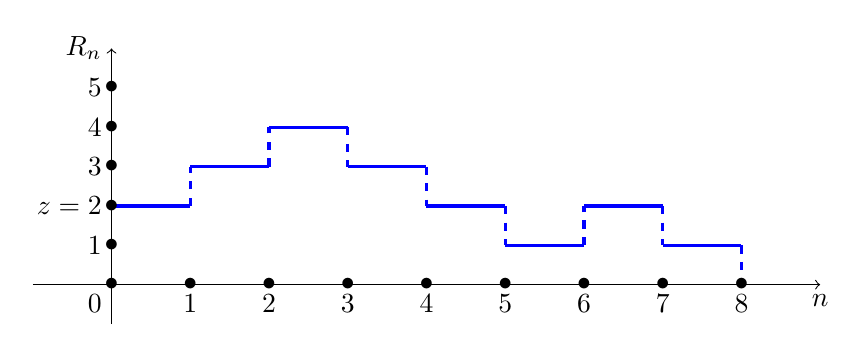
\begin{tikzpicture}
  %Origin and axis
  \coordinate (O) at (0,0);
  \draw[->] (-1,0) -- (9,0) coordinate[label = {below:$n$}] (xmax);
  \draw[->] (0,-0.5) -- (0,3) coordinate[label = {left:$R_n$}] (ymax);
  %Lower linear boundary

 
  %Stochastic process trajectory
  
  \draw (0,0) node[blue,left] {} node{};
  \draw[very thick,blue,-] (0,1) -- (1,1) node[pos=0.5, above] {} ;
  \draw[very thick,dashed,blue] (1,1) -- (1,1.5) node[pos=0.5, right] {};
  \draw[very thick,blue,-] (1,1.5) -- (2,1.5) node[pos=0.5, above] {};
  \draw[very thick,dashed,blue] (2,1.5) -- (2,2) node[pos=0.5, right] {};
  \draw[very thick,blue,-] (2,2) -- (3,2) node[pos=0.5, above] {};
  \draw[very thick,dashed,blue] (3,2) -- (3,1.5) node[pos=0.5, right] {};
  \draw[very thick,blue,-] (3,1.5) -- (4,1.5)node[pos=0.5, above] {};
  \draw[very thick,dashed,blue] (4,1.5) -- (4,1) node[pos=0.5, right] {};  
  \draw[very thick,blue,-] (4,1) -- (5,1) node[pos=0.5, above] {};
  \draw[very thick,dashed,blue] (5,1) -- (5,0.5) node[pos=0.5, right] {};  
  \draw[very thick,blue,-] (5,0.5) -- (6,0.5) node[pos=0.5, above] {};
  \draw[very thick,dashed,blue,-] (6,0.5) -- (6,1) node[pos=0.5, above] {};
   \draw[very thick,blue,-] (6,1) -- (7,1) node[pos=0.5, above] {};
    \draw[very thick,dashed,blue,-] (7,1) -- (7,0.5) node[pos=0.5, above] {};
     \draw[very thick,blue,-] (7,0.5) -- (8,0.5) node[pos=0.5, above] {};
     \draw[very thick,dashed,blue,-] (8,0.5) -- (8,0) node[pos=0.5, above] {};
  %Jump Times
  \draw (1,0) node[black,below] {$1$} node{ \color{black}$\bullet$};
  \draw (2,0) node[black,below] {$2$} node{ \color{black}$\bullet$};
  \draw (3,0) node[black,below] {$3$} node{ \color{black}$\bullet$};
  \draw (4,0) node[black,below] {$4$} node{ \color{black}$\bullet$};
  \draw (5,0) node[black,below] {$5$} node{ \color{black}$\bullet$};
  \draw (6,0) node[black,below] {$6$} node{ \color{black}$\bullet$};
  \draw (7,0) node[black,below] {$7$} node{ \color{black}$\bullet$};
  \draw (8,0) node[black,below] {$8$} node{ \color{black}$\bullet$};
  %Level of the counting process
   \draw (0,0) node[black,below left] {$0$} node{ \color{black}$\bullet$};
   \draw (0,0.5) node[black,left] {$1$} node{ \color{black}$\bullet$};
   \draw (0,1) node[black,left] {$z=2$} node{ \color{black}$\bullet$};
   \draw (0,1.5) node[black,left] {$3$} node{ \color{black}$\bullet$};
   \draw (0,2) node[black,left] {$4$} node{ \color{black}$\bullet$};
   \draw (0,2.5) node[black,left] {$5$} node{ \color{black}$\bullet$};

  % %Aggregated Capital gains
%  \draw (0,1.5) node[blue,below right] {$\mu_1$} node{ \color{blue}$-$};
%  \draw (0,2.25) node[blue,left] {$\mu_2$} node{ \color{blue}$-$};
%  \draw (0,3.75) node[blue,left] {$\mu_3$} node{ \color{blue}$-$};
  %Ruin time = First-crossing time time
%  \draw (5,0) node[black,above right] {${\tau_0}_u$} node{ \color{black}$\times$};
%  \draw[dotted,black] (0,3.28) -- (5,3.28);
%  \draw[dotted,black] (5,0) -- (5,3.28);
\end{tikzpicture}
\label{subfig:ds_RW_time}
}
\hskip1em
\subfloat[Time reversed first hitting problem]{
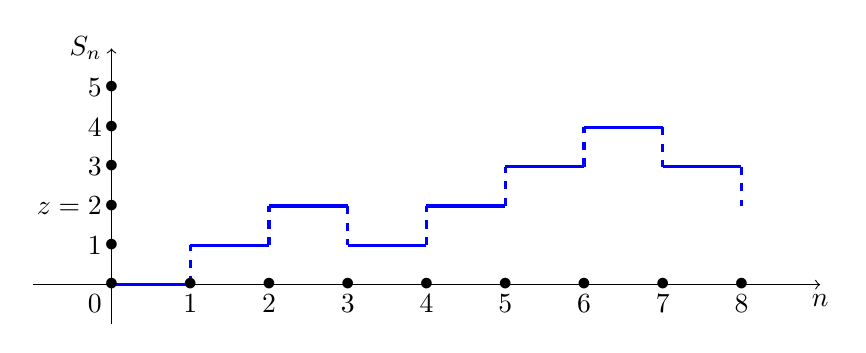
\begin{tikzpicture}
  %Origin and axis
  \coordinate (O) at (0,0);
  \draw[->] (-1,0) -- (9,0) coordinate[label = {below:$n$}] (xmax);
  \draw[->] (0,-0.5) -- (0,3) coordinate[label = {left:$S_n$}] (ymax);
  %Lower linear boundary

 
  %Stochastic process trajectory
  
  \draw (0,0) node[blue,left] {} node{};
  \draw[very thick,blue,-] (0,0) -- (1,0) node[pos=0.5, above] {} ;
  \draw[very thick,dashed,blue] (1,0) -- (1,0.5) node[pos=0.5, right] {};
  \draw[very thick,blue,-] (1,0.5) -- (2,0.5) node[pos=0.5, above] {};
  \draw[very thick,dashed,blue] (2,0.5) -- (2,1) node[pos=0.5, right] {};
  \draw[very thick,blue,-] (2,1) -- (3,1) node[pos=0.5, above] {};
  \draw[very thick,dashed,blue] (3,1) -- (3,0.5) node[pos=0.5, right] {};
  \draw[very thick,blue,-] (3,0.5) -- (4,0.5)node[pos=0.5, above] {};
  \draw[very thick,dashed,blue] (4,0.5) -- (4,1) node[pos=0.5, right] {};  
  \draw[very thick,blue,-] (4,1) -- (5,1) node[pos=0.5, above] {};
  \draw[very thick,dashed,blue] (5,1) -- (5,1.5) node[pos=0.5, right] {};  
  \draw[very thick,blue,-] (5,1.5) -- (6,1.5) node[pos=0.5, above] {};
  \draw[very thick,dashed,blue,-] (6,1.5) -- (6,2) node[pos=0.5, above] {};
   \draw[very thick,blue,-] (6,2) -- (7,2) node[pos=0.5, above] {};
    \draw[very thick,dashed,blue,-] (7,2) -- (7,1.5) node[pos=0.5, above] {};
     \draw[very thick,blue,-] (7,1.5) -- (8,1.5) node[pos=0.5, above] {};
     \draw[very thick,dashed,blue,-] (8,1.5) -- (8,1) node[pos=0.5, above] {};
  %Jump Times
  \draw (1,0) node[black,below] {$1$} node{ \color{black}$\bullet$};
  \draw (2,0) node[black,below] {$2$} node{ \color{black}$\bullet$};
  \draw (3,0) node[black,below] {$3$} node{ \color{black}$\bullet$};
  \draw (4,0) node[black,below] {$4$} node{ \color{black}$\bullet$};
  \draw (5,0) node[black,below] {$5$} node{ \color{black}$\bullet$};
  \draw (6,0) node[black,below] {$6$} node{ \color{black}$\bullet$};
  \draw (7,0) node[black,below] {$7$} node{ \color{black}$\bullet$};
  \draw (8,0) node[black,below] {$8$} node{ \color{black}$\bullet$};
  %Level of the counting process
   \draw (0,0) node[black,below left] {$0$} node{ \color{black}$\bullet$};
   \draw (0,0.5) node[black,left] {$1$} node{ \color{black}$\bullet$};
   \draw (0,1) node[black,left] {$z=2$} node{ \color{black}$\bullet$};
   \draw (0,1.5) node[black,left] {$3$} node{ \color{black}$\bullet$};
   \draw (0,2) node[black,left] {$4$} node{ \color{black}$\bullet$};
   \draw (0,2.5) node[black,left] {$5$} node{ \color{black}$\bullet$};

  % %Aggregated Capital gains
%  \draw (0,1.5) node[blue,below right] {$\mu_1$} node{ \color{blue}$-$};
%  \draw (0,2.25) node[blue,left] {$\mu_2$} node{ \color{blue}$-$};
%  \draw (0,3.75) node[blue,left] {$\mu_3$} node{ \color{blue}$-$};
  %Ruin time = First-crossing time time
%  \draw (5,0) node[black,above right] {${\tau_0}_u$} node{ \color{black}$\times$};
%  \draw[dotted,black] (0,3.28) -- (5,3.28);
%  \draw[dotted,black] (5,0) -- (5,3.28);
\end{tikzpicture}
\label{subfig:time_reversed_ds_RW_time}
}
\end{center}
\caption{Another look at the first hitting time problem.}
\label{fig:time_reversed_double_spending_time}
\end{figure}
Note that \cref{subfig:time_reversed_ds_RW_time} is the reflection of \cref{subfig:ds_RW_time} with respect to the $Y$ axis. We have equivalently
$$
\mathbb{P}_z(\tau_0) = \mathbb{P}(S_k>0,\text{ }1\leq k\leq n|S_n = z, S_0 = 0)\mathbb{P}_0(S_n = z|S_0=0),
$$
and 
$$
\mathbb{P}(S_k>0,\text{ }1\leq k\leq n|S_n = z, S_0 = 0) = \frac{z+(n-z)/2-(n-z)/2}{n} = \frac{z}{n}.
$$
For proof of the ballot theorem, see \citet{Renault2007}. For a general formulation and application to queueing see \citet{Takacs1962}.
\end{remark}
To complete the proof, we just note that 
$$
\mathbb{P}_z(R_n = 0) = \binom{n}{(n-z) / 2}p^{(n-z) / 2}q^{(n
+z) / 2}
$$
as it corresponds to a trajectory of $(R_n)_{n \geq0}$ starting at $R_0 = z$ ending at $0$ made of $(n-z)/2$ upward jumps and $(n+z)/2$ downward one.
\end{proof}
Just like in the previous section, the actual double spending time depends on the value of the random variable $Z = (\alpha -M)_+$.

\subsection{Counting process model}\label{sec:counting_process}
Our aim is to go from the discrete time framework of the previous section to a continuous time. To do so, we will model the length of the blockchain as counting processes. We will consider renewal processes and more specifically Poisson processes. We start by giving some reminders on the exponential distribution and counting processes before studying the double spending time distribution.

\subsubsection{Poisson process, Exponential distributions and friends}\label{sssec:exp_distribution}
\begin{definition}\label{def:counting_process}
A counting process $(N_t)_{t\geq0}$ is a continuous time stochastic process that counts the occurence of an event over time such that
\begin{equation*}
N_0=0\text{ and }N_t=\sum_{k=1}^{+\infty}\mathbb{I}_{T_k\leq t}.
\end{equation*}
where $T_1,T_2,T_3,\ldots$ denote the arrival times, with the convention that $T_0=0$. Let $\Delta^T_0,\Delta^T_1,\Delta^T_2,\ldots$ be the sequence of inter-arrival times defined as
$$
\Delta^T_k=T_{k+1}-T_{k}\text{, }k=0,1,2\ldots.
$$
\end{definition}
A trajectory of a counting process is given in 
\begin{figure}[!h]
\begin{center}
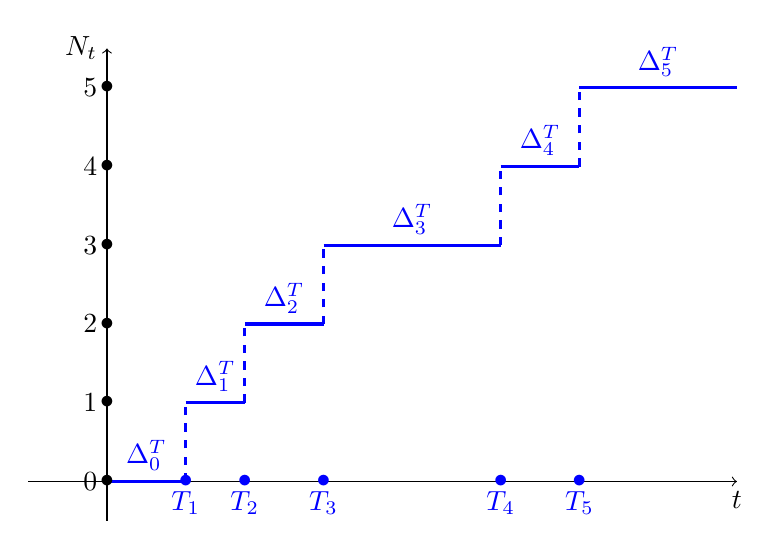
\begin{tikzpicture}[scale=1]
  %Origin and axis
  \coordinate (O) at (0,0);
  \draw[->] (-1,0) -- (8,0) coordinate[label = {below:$t$}] (xmax);
  \draw[->] (0,-0.5) -- (0,5.5) coordinate[label = {left:$N_t$}] (ymax);
  %Lower linear boundary


  %Stochastic process trajectory

  \draw (0,0) node[blue,left] {} node{};
  \draw[very thick,blue,-] (0,0) -- (1,0) node[pos=0.5, above] {$\Delta^T_0$} ;
  \draw[very thick,dashed,blue] (1,0) -- (1,1) node[pos=0.5, right] {};
  \draw[very thick,blue,-] (1,1) -- (1.75,1) node[pos=0.5, above] {$\Delta^T_1$};
  \draw[very thick,dashed,blue] (1.75,1) -- (1.75,2) node[pos=0.5, right] {};
  \draw[very thick,blue,-] (1.75,2) -- (2.75,2) node[pos=0.5, above] {$\Delta^T_2$};
  \draw[very thick,dashed,blue] (2.75,2) -- (2.75,3) node[pos=0.5, right] {};
  \draw[very thick,blue,-] (2.75,3) -- (5,3)node[pos=0.5, above] {$\Delta^T_3$};
  \draw[very thick,dashed,blue] (5,3) -- (5,4) node[pos=0.5, right] {};
  \draw[very thick,blue,-] (5,4) -- (6,4) node[pos=0.5, above] {$\Delta^T_4$};
  \draw[very thick,dashed,blue] (6,4) -- (6,5) node[pos=0.5, right] {};
  \draw[very thick,blue,-] (6,5) -- (8,5) node[pos=0.5, above] {$\Delta^T_5$};
  %Jump Times
  \draw (1,0) node[blue,below] {$T_1$} node{ \color{blue}$\bullet$};
  \draw (1.75,0) node[blue,below] {$T_2$} node{ \color{blue}$\bullet$};
  \draw (2.75,0) node[blue,below] {$T_3$} node{ \color{blue}$\bullet$};
  \draw (5,0) node[blue,below] {$T_4$} node{ \color{blue}$\bullet$};
  \draw (6,0) node[blue,below] {$T_5$} node{ \color{blue}$\bullet$};
  %Level of the counting process
   \draw (0,0) node[black,left] {$0$} node{ \color{black}$\bullet$};
   \draw (0,1) node[black,left] {$1$} node{ \color{black}$\bullet$};
   \draw (0,2) node[black,left] {$2$} node{ \color{black}$\bullet$};
   \draw (0,3) node[black,left] {$3$} node{ \color{black}$\bullet$};
   \draw (0,4) node[black,left] {$4$} node{ \color{black}$\bullet$};
   \draw (0,5) node[black,left] {$5$} node{ \color{black}$\bullet$};
\end{tikzpicture}
\end{center}
\caption{Trajectory of the counting process $(N_t)_{t\geq0}$.}
\label{fig:trajectory_counting_process}
\end{figure}
\begin{definition}\label{def_poisson_process}
A Poisson process $(N_t)_{t\geq0}$ is a counting process whose inter-arrival times are \iid exponential random variables.
\end{definition}
\begin{remark}\label{def_renewal_process}
A Poisson process belongs to the family renewal processes which are counting process with \iid inter-arrival times.
\end{remark}
\begin{definition}\label{def:exp_dist}
A random variable $X$ is exponentially distributed $X\sim\ExpDist(\lambda)$ if it has \pdf
$$
f_X(x) =\begin{cases} 
\lambda\e^{-\lambda x},&\text{ if }x>0,\\
0,&\text{ otherwise}.
\end{cases}
$$
\end{definition}
For some reasons, we need to introduce the joint distribution of the order statistics of a uniform random sample.
\begin{prop}\label{def:uniform_OS_dist}
Let $U_1,\ldots, U_n$ be a sample of \iid uniform random variables on $(a,b)$. Denote by 
$$
U_{(1)}\leq U_{(2)}\leq\ldots\leq U_{(n)}
$$
the order statistics of such a sample. The joint distribution of $(U_{(1)},\ldots,  U_{(n)})$ is given by 
$$
f_{(U_{(1)},\ldots, U_{(n)})}(u_1,\ldots, u_n)=\frac{n!}{(b-a)^n}\mathbb{I}_{a<u_1<\ldots< u_n<b}(u_1,\ldots, u_n).
$$
and we denote $(U_{(1)},\ldots,  U_{(n)})\sim \text{OS}_n([a,b])$
\end{prop}
\begin{proof}
Let $g:\mathbb{R}^n\mapsto \mathbb{R}_+$ be measurable and bounded. We have that
$$
\mathbb{E}[g(U_{(1)},\ldots,U_{(n)})]=\mathbb{E}\left[\sum_{\sigma\in\mathcal{S}_n}
g(U_{\sigma(1)},\ldots,U_{\sigma(n)})
\mathbb{I}_{U_{\sigma(1)} <\ldots< U_{\sigma(n)}}
\right]
$$
where $\mathcal{S}_n$ the set of all the permutation of $\{1,\ldots,n \}$. We note that
\begin{eqnarray*}
\mathbb{E}\left[g(U_{\sigma(1)},\ldots,U_{\sigma(n)})
\mathbb{I}_{U_{\sigma(1)} <\ldots< U_{\sigma(n)}}
\right]&=& \mathbb{E}\left[g(U_{1},\ldots,U_{n})
\mathbb{I}_{U_{1} <\ldots< U_{n}}\right]\\
&=&\int_{\mathbb{R}^{n}}g(u_{1},\ldots,u_{n})
\mathbb{I}_{u_{1} <\ldots< u_{n}}\frac{1}{(b-a)^n}\text{d}\lambda_{n}(u_1,\ldots, u_n).
\end{eqnarray*}
It then follows that
$$
\mathbb{E}[g(U_{(1)},\ldots,U_{(n)})]=\int_{\mathbb{R}^{n}}g(u_{1},\ldots,u_{n})
\mathbb{I}_{u_{1} <\ldots< u_{n}}\frac{n!}{(b-a)^n}\text{d}\lambda_{n}(u_1,\ldots, u_n).
$$
\end{proof}
We require some additional result about the gamma distribution.
\begin{prop}\label{prop:erlang_dist}
Let $\Delta^T_1,\ldots, \Delta^T_n$ be \iid exponential $\text{Exp}(\lambda)$ random variables, define the sequence $T_k=\sum_{i=1}^{k}\Delta^T_i, k=1,\ldots, n$.
\begin{enumerate}
\item The $T_{k}$'s have an Erlang distribution. We denote by $T_{k}\sim\text{Erl}(k,\lambda)$ with 
$$
f_{T_k}(t)=\frac{t^{k-1}e^{-\lambda t}\lambda^k}{(k-1)!},\text{ }t>0.
$$
\item The joint distribution of $(T_1,\ldots, T_n)$ has \pmf given by
$$
f_{(T_1,\ldots, T_n)}(t_1,\ldots, t_n)=\lambda^n e^{-\lambda t_n }\mathbb{I}_{0<t_1<\ldots< t_n}(t_1,\ldots, t_n)
$$
\item $[(T_1,\ldots, T_n)|T_{n+1}=t]\sim \text{OS}_{n}([0,t])$
\end{enumerate}
\end{prop}
\begin{proof}
\begin{enumerate}
\item We use induction on $k\geq1$. For $k=1$ we have that $\Delta^T_1= T_1$ so the property holds. Assume that the property hold true for some $k$ and consider $k+1$. We note that $T_{k+1}=T_k+\Delta^T_{k+1}$ then
\begin{eqnarray*}
f_{T_{k+1}}(t)&=&\int_{0}^{t}f_{T_k}(x)f_{\Delta^T_{k+1}}(t-x)\text{d}x\\
&=&\int_{0}^{t}\frac{x^{k-1}e^{-\lambda x}\lambda^k}{(k-1)!}\lambda e^{-\lambda(t-x)}\text{d}x\\
&=&\frac{e^{-\lambda t}\lambda^{k+1}}{(k-1)!}\frac{t^k}{k}=\frac{t^k e^{-\lambda t}\lambda^{k+1}}{k!}.
\end{eqnarray*}
\begin{exercise}
Can you propose another way to show this result? Without using induction.
\end{exercise}
\item Let $g:\mathbb{R}^n\mapsto \mathbb{R}_+$ be meaurable and bounded, we have
\begin{eqnarray*}
\mathbb{E}[g(T_{1},\ldots,T_n)]&=& \mathbb{E}[g(\Delta^T_{1},\Delta^T_1+\Delta^T_2\ldots,\Delta^T_1+\ldots+ \Delta^T_n)]\\
&=&\int_{\mathbb{R}^n}g(t_{1},\ldots,t_1+\ldots+ t_n)f_{(\Delta^T_{1},\ldots,\Delta^T_n)}(t_1,\ldots,t_n)\text{d}\lambda_n(t_{1},\ldots,t_n)\\
\end{eqnarray*}
Let us apply the following change of variable 
$$
\Phi:(u_{1},\ldots,u_n)\mapsto(u_1, u_{2}-u_1,\ldots,u_n-u_{n-1}):=(t_1,\ldots, t_n),$$
minding the change in the integration domain as 
$$
\Phi(\mathbb{R}_+\times ]u_1,\infty[\times \ldots\times ]u_{n-1},\infty[) = \mathbb{R}^n 
$$
and the Jacobian $\left|\frac{\text{d}\Phi}{\text{d}u}\right|=1$. It follows that
$$
\mathbb{E}[g(T_{1},\ldots,T_n)]=\int_{\mathbb{R}^n} g(u_1,\ldots, u_n)\lambda^{n}e^{-\lambda u_n}\mathbb{I}_{0<u_1<\ldots<u_n}(u_1,\ldots, u_n)\text{d}\lambda_{n}(u_1,\ldots, u_n).
$$
\item We have that 
\begin{eqnarray*}
f_{T_1,\ldots, T_n|T_{n+1}}(t_1,\ldots,t_n|t)
&=&\frac{f_{T_1,\ldots, T_n,T_{n+1}}(t_1,\ldots,t_n,t)}{f_{T_{n+1}(t)}}\\
&=&\frac{n!}{t^n}\mathbb{I}_{0<t_1<\ldots< t_n<t}(t_1,\ldots, t_n, t).
\end{eqnarray*}
\end{enumerate}
\end{proof}
The fact that the Poisson process is a Levy process will be useful later on, so here it is
\begin{prop}
The following statements are equivalent
\begin{enumerate}
\item $(N_t)_{t\geq 0}$ is a Poisson process
\item The stochastic process $(N_t)_{t\geq 0}$ has
\begin{itemize}
\item[(i)] independent increments, it means that for $0<t_1\leq\ldots\leq t_n$, the random variables
$N_{t_1},N_{t_2}-N_{t_1},\ldots,N_{t_{n}}-N_{t_{n-1}}$
are independent.
\item[(ii)] stationnary increments in the sense that the event frequency distribution over some time period of duration $s>0$ only depends on $s$. Indeed, we have that 
$$
N_{t+s}-N_t\sim\PoissonDist(\lambda s),\text{ for }s,t\geq 0.
$$
\end{itemize}
\end{enumerate}
The stochastic processes with independent and stationnary increments are called Levy processes.
\end{prop}
\begin{proof}
\underline{$1 \Rightarrow 2$}\\
Assume that $(N_t)_{t\geq0}$ is a Poisson process and let $0<t_1<\ldots <t_n$ be some times. Consider the folowing probability 
$$
\mathbb{P}\left(N_{t_1} = j_1, N_{t_2}-N_{t_1} = j_2,\ldots, N_{t_n}-N_{t_{n-1}} = j_n\right)
$$
such that $j_1,\ldots, j_n\in \mathbb{N}$. We can rewrite it as 
$$
\mathbb{P}\left(T_{k_1}\leq t_1<T_{k_1+1}, T_{k_2}\leq t_2<T_{k_2+1},\ldots, T_{k_n} \leq t_n<T_{k_n+1}\right),
$$
where $k_i = j_1 + \ldots +j_i, i = 1,\ldots, n$. Conditionning with respect to  $T_{k_n+1}$ yields
\begin{eqnarray*}
&&\mathbb{P}\left(T_{k_1}\leq t_1<T_{k_1+1}, T_{k_2}\leq t_2<T_{k_2+1},\ldots, T_{k_n}\leq t_n<T_{k_n+1}\right)\\
&=&\int_{t_n}^{+\infty}\mathbb{P}\left(T_{k_1}<t_1<T_{k_1+1}, T_{k_2}<t_2<T_{k_2+1},\ldots, T_{k_n}<t_n|T_{k_n +1}=t\right)f_{T_{k_n+1}}(t)\text{d}\lambda(t)\\
&=& \int_{t_n}^{+\infty}\binom{k_n}{j_1,\ldots, j_n}\left(\frac{t_1}{t}\right)^{j_1}\left(\frac{t_2-t_1}{t}\right)^{j_2}\ldots \left(\frac{t_n-t_{n-1}}{t}\right)^{j_n}\frac{e^{-\lambda t}t^{k_n}\lambda^{k_n + 1}}{k_n!}\text{d}\lambda(t)\\
&=&\frac{e^{-\lambda t_1}\left(t_1\right)^{j_1}}{j_1!}\frac{\left(t_2-t_1\right)^{j_2}e^{-\lambda(t_2 - t_1)}}{j_2!}\ldots \frac{\left(t_n-t_{n-1}\right)^{j_n}e^{-\lambda(t_n - t_{n-1})}}{j_n!}
\end{eqnarray*}
From the second to the third equality we simply ask that amomg $k_n$ uniform random variables $j_1$ fall inside $(0,t_1)$, $j_2$ fall inside $(t_1,t_2)$, etc...


\noindent \underline{$2 \Rightarrow 1$}\\
We aim at showing that $(T_1,\ldots, T_n)$ has \pdf given by
\begin{equation}\label{eq:joint_density_arrival_times}
f_{T_1,\ldots, T_n}(t_1,\ldots, t_n)=\lambda^n e^{-\lambda t_n}\mathbb{I}_{0< t_1<\ldots<t_n}.
\end{equation}
Let $t_1,\ldots, t_n$ and $h$ be nonnegative real numbers such that
$$
t_1<t_1+h<t_2<\ldots<t_n<t_n+h,
$$ 
We have
\begin{eqnarray*}
&&\mathbb{P}(t_1<T_1<t_1+h,\ldots,t_n<T_1<t_n+h)\\
&=&\mathbb{P}(N_{t_1}=0,N_{t_1+h}-N_{t_1}=1,\ldots,N_{t_n}-N_{t_{n-1}+h}=0,N_{t_n+h}-N_{t_n}\geq 1)\\
&=&e^{-\lambda t_1}e^{-\lambda h}\lambda h e^{-\lambda [t_2-(t_1+h)]}e^{-\lambda h}\lambda h\ldots e^{-\lambda [t_n-(t_{n-1}+h)]}[1-e^{-\lambda h}] \\
&=&e^{-\lambda t_n}\lambda^{n-1}h^{n-1}[1-e^{-\lambda h}]\\
\end{eqnarray*}
Divide by $h^{n}$ and let $h$ go to $0$ to get \eqref{eq:joint_density_arrival_times}. After applying a change of variable (reciprocal of that used in the proof of \cref{prop:erlang_dist}) to recover the joint distribution of $(\Delta^{T}_1, \ldots, \Delta^{T}_n)$, we see that the later is actually that of an \iid sample of size $n$ of exponential random variables.
\end{proof}
Last but not the lis, we establish the order statistic property of the Poisson process.
\begin{prop}
Provided that$\{N_t=n\}$, The jump times $T_1,\ldots,T_n$ have the same distribution as the order statistic of an \iid sample of $n$ uniform random variable on $(0,t)$, namely it holds that
$$
[T_1,\ldots,T_n|N_t=n]\sim \left(U_{(1)}(0,t),\ldots, U_{(n)}(0,t)\right).
$$
\end{prop}
\begin{proof}
We have
\begin{eqnarray*}
&&\mathbb{E}\left[g(T_1,\ldots, T_n)|N_t = n\right]\\
&=&\frac{\mathbb{E}\left[g(T_1,\ldots, T_n)\mathbb{I}_{N_t = n}\right]}{\mathbb{P}(N_t = n)}\\
&=&\frac{n!}{e^{-\lambda t}(\lambda t)^n}\int_{\mathbb{R}^{n+1}}g(t_1,\ldots, t_n)\mathbb{I}_{t_n\leq t<t_{n+1}}(t_n,t_{n+1})f_{T_1,\ldots, T_{n+1}}(t_1,\ldots, t_{n+1})\text{d}\lambda_{n+1}(t_1,\ldots, t_{n+1})\\
&=&\frac{n!}{e^{-\lambda t}(\lambda t)^n}\int_{\mathbb{R}^{n}}\int_{t}^{+\infty}g(t_1,\ldots, t_n)\mathbb{I}_{0<t_1<\ldots t_n\leq t}(t_1,\ldots,t_{n})\lambda^{n+1} e^{-\lambda t_{n+1}}\text{d}\lambda_{n+1}(t_1,\ldots, t_{n+1})\\
&=&\frac{n!}{e^{-\lambda t}(\lambda t)^n}\int_{\mathbb{R}^{n}}\int_{t}^{+\infty}g(t_1,\ldots, t_n)\mathbb{I}_{0<t_1<\ldots t_n\leq t}(t_1,\ldots,t_{n})\lambda^{n} \text{d}\lambda_{n}(t_1,\ldots,t_n)\e^{-\lambda t}\\
 &=&\int_{\mathbb{R}^{n}}g(t_1,\ldots, t_n)\frac{n!}{t^n}\mathbb{I}_{0<t_1<\ldots t_n\leq t}(t_1,\ldots,t_{n})\text{d}\lambda(t_1,\ldots,t_{n} ).
\end{eqnarray*}
\end{proof}
\noindent The order statistic property of the Poisson process will be useful to solve the first hitting time problem arising later on. To fully benefit from this nice property, we need to introduce Appell and Abel-Gontcharov polynomials.\\

\noindent Let $U=\{u_i, \, i\geq 1\}$ be a non-decreasing sequence of real numbers. To $U$ is attached a (unique) family of Appell polynomials of degree $n$ in $x$, $\{A_{n}(x\vert U),\, n\geq 0\}$ defined as follows.
\begin{definition} 
Starting with $A_0(x\vert U)=1$, the $A_n(x\vert U)$'s satisfy the differential equations
\begin{equation}\label{eq:DifferentialEquationAppellPolynomial}
A_{n}^{(1)}(x|U)=nA_{n-1}(x|U),  
\end{equation}
with the border conditions
\begin{equation}\label{eq:Border AppellPolynomial}
A_{n}(u_{n}|U)=0, \quad n\geq 1.
\end{equation}
So, each $A_n$ has the integral representation
\begin{equation}\label{eq:IntegralRepresentationAppellPolynomials}
A_{n}(x|U)=n!\int_{u_{n}}^{x}\left[\int_{u_{n-1}}^{y_{n}}\text{d}y_{n-1} \ldots \int_{u_{1}}^{y_{1}}\text{d}y_{1}\right]\text{d}y_{n}, \quad n\geq 1.
\end{equation}
\end{definition}

In parallel, to $U$ is attached a (unique) family of Abel-Gontcharov (A-G) polynomials of degree $n$ in $x$, $\{G_{n}(x\vert U),\, n\geq 0\}$.
\begin{definition} 
Starting with $G_0(x\vert U)=1$, the $G_n(x\vert U)$'s satisfy the differential equations
\begin{equation}\label{eq:DifferentialEquationAGPolynomials}
G_n^{(1)}(x|U)=nG_{n-1}(x|{\cal E}U), 
\end{equation}
where ${\cal E}U$ is the shifted family $\{u_{i+1}, \, i\geq 1\}$, and with the border conditions
\begin{equation}\label{eq:Border AGPolynomial}
G_{n}(u_{1}|U)=0, \quad  n\geq 1.
\end{equation}
So, each $G_n$ has the integral representation
\begin{equation}\label{eq:IntegralRepresentationAGPolynomials}
G_{n}(x|U)=n!\int_{u_{1}}^{x}\left[\int_{u_{2}}^{y_{1}}\text{d}y_{2} \ldots \int_{u_{n}}^{y_{n-1}}\text{d}y_{n}\right]\text{d}y_{1}, \quad n\geq 1.
\end{equation}
\end{definition}
\noindent The Appell and A-G polynomials are closely related through the identity
\begin{equation}\label{eq:link_AG_Appell}
G_{n}(x|u_{1},\ldots,u_{n})=A_{n}(x|u_{n},\ldots,u_{1}), \quad n\geq 1.
\end{equation}
The two families (i.e. for all $n\geq 0$), however, are distinct and enjoy different properties. From \eqref{eq:IntegralRepresentationAppellPolynomials} and \eqref{eq:IntegralRepresentationAGPolynomials}, it is clear that the polynomials $A_n$ and $G_n$ can be interpreted in terms of the joint distribution of the vector $(U_{1:n},\ldots,U_{n:n})$. 
\begin{prop}
For $0\leq u_1 \leq \ldots \leq u_{n} \leq x \leq 1$,
\begin{equation}\label{eq:ProbabilisticInterpretationAppellPolynomials}
P[U_{(1)} \geq u_1, \ldots, U_{(n)} \geq u_{n}\, \mbox{ and }\, U_{(n)}\leq x]= 
A_n(x \vert u_1, \ldots, u_{n}), \quad n\geq1.
\end{equation}
For $0\leq x \leq u_1 \leq \ldots \leq u_{n} \leq 1$,
\begin{equation}\label{eq:ProbabilisticInterpretationAGPolynomials}
P[U_{(1)} \leq u_1, \ldots, U_{(n)} \leq u_{n}\, \mbox{ and }\, U_{(1)}\geq x]
= (-1)^n \, G_n(x \vert u_1, \ldots, u_{n}), \quad n\geq 1.
\end{equation}
\end{prop}
The representations \eqref{eq:ProbabilisticInterpretationAppellPolynomials} and \eqref{eq:ProbabilisticInterpretationAGPolynomials} will play a key role for solving first-hitting problem that involve Poisson processes. Numerically, it will be necessary to evaluate some special values of the polynomials. To this end, it is convenient to use the following recusive relations. 
\begin{prop} 
The Appell polynomials are computed through the expansion
\begin{equation}\label{eq:appell_polynomials_recursion_1}
A_{n}(x|U)=\sum_{k=0}^{n}\binom{n}{k}A_{n-k}(0|U)x^{k}, \quad n\geq 1,
\end{equation}
where the $A_{n}(0|U)$'s are obtained recursively from 
\begin{equation}\label{eq:appell_polynomials_recursion_2}
A_{n}(0|U)=-\sum_{k=1}^{n} \binom{n}{k} A_{n-k}(0|U)u_{n}^{k}, \quad n\geq1.
\end{equation}
The A-G polynomials are computed through the recursion
\begin{equation}\label{eq:recursion_AG_polynomials}
G_{n}(x|U)=x^{n}-\sum_{k=0}^{n-1} \binom{n}{k} u_{k+1}^{n-k} G_{k}(x|U), \quad n\geq 1.
\end{equation}
\end{prop}
\begin{proof}
The Maclaurin expansion of $A_n(x|U)$ gives \eqref{eq:appell_polynomials_recursion_1} as
$$
A_n(x|U) = \sum_{k = 0}^n\frac{A_n^{(k)}(x|U)}{k!}x^k = \sum_{k = 0}^n\binom{n}{k}A_{n-k}(x|U)x^k.
$$
Evaluation at $x = u_n$ then provides \eqref{eq:appell_polynomials_recursion_2}. Regarding \eqref{eq:recursion_AG_polynomials}, first note that 
$$
G_n^{(k)}(u_{k+1}|U) = \begin{cases}
1,&\text{ if }k = n,\\
0,&\text{ otherwise.}
\end{cases}
$$
Any polynomials $R(x)$ of degree $n$ can therefore be written as 
$$
R(x)=\sum_{k = 0}^n\frac{R^{(k)}(u_{k+1})}{k!}G_k(x|U).
$$
By expanding $x^n$ one gets \eqref{eq:recursion_AG_polynomials}.
\end{proof}
Hereafter are a couple of useful properties
\begin{prop}\label{prop:Appell_AG_polynomials_properties}
\begin{enumerate}
\item For any $a,b\in \mathbb{R}$, it holds that
\begin{equation}
A_{n}(x|a+bU) = b^n A_n\left((x-a)/b \, |U\right), \quad n\geq 1, \label{eq:LinearTransform}
\end{equation}
with the same identity for $G_n$.
\item Let $\{X_{n}\text{ , }n\geq1\}$ be a sequence of \iid nonnegative random variables, of partial sums $S_{n}=\sum_{k=1}^{n}X_{k}$ with $S_0=0$. Then, for $n\geq 1$,
\begin{eqnarray}
&&\mathbb{E} \left[A_{n}(x|S_{1},\ldots,S_{n})\vert S_{n}\right] = x^{n-1}(x-S_{n}), \label{eq:ExplicitExpressionPartialSumsAppellPolynomials}\\
&&\mathbb{E}\left[G_{n}(x|S_{0},\ldots,S_{n-1})\vert S_{n}\right] = x(x-S_{n})^{n-1}.    \label{eq:ExplicitExpressionPartialSumsAGPolynomials}
\end{eqnarray}
\end{enumerate} 
\end{prop}
\begin{proof}
\begin{enumerate}
  \item Let us use induction on $n\geq1$. Take $n = 1$, we have
  $$
  A_1(x|a + bu_1) = \int_{a+bu_1}^{x} A_1'(y|a+bu_1)\text{d}y = x - a - bu_1 
  $$
  and 
   $$
  A_1(x|u_1) = x-u_1.
  $$
  The property holds for $n = 1$. Assume that it holds true for some $n$ and consider $n+1$. We have
  \begin{eqnarray*}
  A_{n+1}(x|a+bU) &=& \int^{x}_{a+b u_{n+1}}A_{n+1}'(y|a+bU)\text{d}y\\
  &=& \int^{x}_{a+b u_{n+1}}nA_{n}(y|a+bU)\text{d}y\\
  &=&b^n\int^{x}_{a+b u_{n+1}}nA_{n}\left(\frac{y-a}{b}\Big|U\right)\text{d}y\\
  &=&b^{n+1}n\int^{\frac{x-a}{b}}_{u_{n+1}}A_{n}\left(z\Big|U\right)\text{d}y\\
  &=&b^{n+1}\int^{\frac{x-a}{b}}_{u_{n+1}}A_{n+1}'\left(z\Big|U\right)\text{d}y\\
  &=&b^{n+1}A_{n+1}\left(\frac{x-a}{b}\Big|U\right),
  \end{eqnarray*}
  so the property holds for $n+1$. No need to do the job for the $G_n(.|U)$'s thanks to \eqref{eq:link_AG_Appell}.
\item Again induction on $n\geq1$. Take $n = 1$, we have
$$
\mathbb{E}[A_1(x|S_1)|S_1] = x-S_1
$$
Assume that the result holds true for some $n$ and consider $n+1$. We have 
\begin{eqnarray*}
\mathbb{E}\left[A_{n+1}(x|S_1,\ldots, S_n,S_{n+1})|S_{n+1}\right]&=&\mathbb{E}\left[\int_{S_{n+1}}^x A_{n+1}'(y|S_1,\ldots, S_n,S_{n+1})\text{d}y|S_{n+1}\right]\\
&=&\int_{S_{n+1}}^x\mathbb{E}\left[ A_{n+1}'(y|S_1,\ldots, S_n,S_{n+1})|S_{n+1}\right]\text{d}y\\
&=&(n+1)\int_{S_{n+1}}^x\mathbb{E}\left[A_{n}(y|S_1,\ldots, S_n)|S_{n+1}\right]\text{d}y\\
&=&(n+1)\int_{S_{n+1}}^x\mathbb{E}\left\{\mathbb{E}\left[A_{n}(y|S_1,\ldots, S_n)|S_n,S_{n+1}\right]S_{n+1}\right\}\text{d}y\\
&=&(n+1)\int_{S_{n+1}}^x\mathbb{E}\left\{\mathbb{E}\left[A_{n}(y|S_1,\ldots, S_n)|S_n\right]|S_{n+1}\right\}\text{d}y\\
&=&(n+1)\int_{S_{n+1}}^x\mathbb{E}\left[y^{n-1}(y-S_n)|S_{n+1}\right]\text{d}y\\
&=&(n+1)\int_{S_{n+1}}^xy^n-\frac{n}{n+1}S_{n+1}y^{n-1} \text{d}y\\
&=&x^n(x-S_{n+1})\\
\end{eqnarray*}
For identity \eqref{eq:ExplicitExpressionPartialSumsAGPolynomials}, write 
\begin{eqnarray*}
\mathbb{E}\left[G_{n}(x|S_0,\ldots, S_{n-1})|S_{n}\right]&=&\mathbb{E}\left[G_{n}(x-S_n|S_0 - S_n,\ldots, S_{n-1}-S_n)|S_{n}\right]\\
&=&(-1)^n\mathbb{E}\left[G_{n}(S_n-x|S_n,\ldots, S_{n}-S_{n-1})|S_{n}\right]\\
&=&(-1)^n\mathbb{E}\left[A_{n}(S_n-x|S_{n}-S_{n-1},\ldots, S_n)|S_{n}\right]\\
&=&(-1)^n(S_n-x -S_n)(S_n-x)^{n-1}\\
&=&x(x-S_n)^{n-1}.\\
\end{eqnarray*}
\end{enumerate}
\end{proof}

\subsubsection{A tiny bit of insurance risk theory}\label{sssec:insurance_risk_theory}
In what follows we will use classical result from insurance risk theory and so we have to provide some context. The financial reserve of a nonlife insurance company can be modelled by a continuous time stochastic process $(R_t)_{t\geq0}$ defined as 
\begin{equation}\label{eq:risk_process}
R_t = u + P_t - L_t,\text{ }t\geq0
\end{equation}
where 
\begin{itemize}
  \item $R_0 = u>0$ are the initial reserves,
  \item $(P_t)_{t\geq0}$ is the premium income process,
  \item $(L_t)_{t\geq0}$ is the liability of the insurance company, that is the sum of all the compensations paid to to the policyholders.
\end{itemize}
The classical assumes that the premium are collected linearly in times at some rate $c$ per time unit. Namely, we have 
$$
P_t = c\times t.
$$
The number of claims is governed by a counting process $(N_t)_{t\geq0}$, usually a standard Poisson process with intensity $\lambda$. To each claim is associated a randomly sized compensation distributed as $U$. The claim sizes $U_1,U_2,\ldots$ form a sequence of \iid random variables independent from $N_t$. We therefore have 
$$
L_t = \sum_{k = 1}^{N_t}U_k.
$$
The name of the game is to compute the ruin probabilities 
\begin{equation}\label{eq:ruin_probabilities}
\psi(u,T) = \mathbb{P}(\tau_0 \leq T),\text{ and }\psi(u) = \mathbb{P}(\tau_0 < \infty),
\end{equation} 
where $\tau_0 = \inf\{t\geq0\text{ ; }R_t \leq 0\}$ is the ruin time. This first hitting time problem is illustrated on \cref{fig:ruin_time_CL}
\begin{figure} 
\begin{center}
\begin{tikzpicture}
  %Origin and axis
  \coordinate (O) at (0,0);
  \draw[->] (-0.5,0) -- (5.5,0) coordinate[label = {below:$t$}] (xmax);
  \draw[->] (0,-0.5) -- (0,4) coordinate[label = {right:$R_t$}] (ymax);
   %Initial reserves
  \draw (0,2) node[black,left] {$z$} node{};
 % % %Length of the honest chain
  \draw[thick, blue,-] (0,2) -- (2,3) node[pos=0.5, above] {};
  \draw[thick, dashed, blue] (2,3) -- (2,1) node[pos=0.5, left] {\color{black}$U_1$};
  \draw[thick, blue] (2,1) -- (3,1.5) node[pos=0.5, above] {};
  \draw[thick, dashed, blue] (3,1.5) -- (3, 0.5) node[pos=0.5, left] {\color{black}$U_2$};
  \draw[thick, blue] (3,0.5) -- (5, 1.5) node[pos=0.5, above] {};
   \draw[thick, dashed, blue] (5,1.5) -- (5, -0.5) node[pos=0.5,above left] {\color{black}$U_3$};

  %Block finding Times 
  \draw (2,0) node[black,below] {$T_1$} node{ \color{black}$\bullet$};
  \draw (3,0) node[black,below] {$T_2$} node{ \color{black}$\bullet$};
  \draw (5,0) node[black,below left] {$\tau_0$} node{ \color{black}$\bullet$};
\end{tikzpicture}
\end{center}
\label{fig:ruin_time_CL}
\caption{Illustration of the classical insurance ruin problem}
\end{figure}
This enables to select an initial reserves level $u$ so that the ruin probability is low enough. The premium rate is usually set to compensate the losses due to claims with 
$$
\mathbb{E}(P_t) = (1+\eta)\mathbb{E}(L_t)\text{ or  equivalently } c = (1+\eta)\lambda\mathbb{E}(U).
$$
Define the claim surplus process as
$$
S_t = u - R_t = L_t-P_t,\text{ }t\geq 0.
$$
The following result is the counterpart of \cref{lem:wald_martingale_RW} for Lévy processes.
\begin{prop}\label{prop:wald_martingale_levy}
If $(S_t)_{t\geq0}$ is a L\'evy process then
$$
M_t = \exp\left[s S_t-t\kappa(s)\right]\text{, }t\geq0,
$$
where $\kappa(s)=\log\mathbb{E}\left(e^{s S_1}\right)$, is a Martingale.
\end{prop}
The infinite time horizon ruin probability may be evaluated using the following result.
\begin{prop}\label{prop:ruin_proba_levy}
If $S_t\overset{\textbf{a.s.}}{\rightarrow} -\infty$, and there exists $\gamma>0$ such that $\left(e^{\gamma S_t}\right)_{t\geq0}$ is a martingale then
$$
\mathbb{P}(\tau_0<\infty)=\frac{e^{-\gamma u}}{\mathbb{E}\left[e^{\gamma \xi(u)}|\tau_0<\infty\right]},
$$
where $\xi(u)=S_{\tau_0}-u$ denotes the deficit at ruin.
\end{prop}
\begin{proof}
We apply the optionnal stopping theorem on $(e^{\gamma S_t})_{t\geq0}$ at time $T\land \tau_0$ for some $T>0$ to get 
\begin{eqnarray*}
1 = \mathbb{E}\left(\e^{\gamma S_0}\right)&=& \mathbb{E}\left(\e^{\gamma S_{T\land \tau_0}}\right)\\  
&=& \mathbb{E}\left(\e^{\gamma S_{\tau_0}}\mathbb{I}_{\tau_0\leq T} + \e^{\gamma S_{T}}\mathbb{I}_{\tau_0> T}\right).\\
\end{eqnarray*} 
Letting $T\rightarrow\infty$ yields\footnote{Thanks to $S_t\rightarrow -\infty$, monotone and dominated convergence.}
\begin{eqnarray*}
1 &=&\mathbb{E}\left(\e^{\gamma S_{\tau_0}}\mathbb{I}_{\tau_0<\infty}\right)\\
&=&\e^{\gamma u}\mathbb{E}\left(\e^{\gamma \xi(u))}|\tau_0<\infty\right)\psi(u).
\end{eqnarray*} 
\end{proof}
We will use \cref{prop:ruin_proba_levy} to derive the double spending probability within a continuous time framework in the next sections.
\subsubsection{Double spending probability}\label{sssec:double_spending_counting_process_dsp}
The \textit{Proof-of-Work} protocol implies a steady block arrival, every $10$ minnutes for the bitcoin blockchain. Each trial (of the network) for mining a block is independent of the others and leads to a success with very small probability, the overall number of successes is binomially distributed, very well approximated by a
Poisson random variable. This justifies the Poisson process assumption made in the sequel to model the block arrival.\\

\noindent Denote by $(z+ N_t)_{t\geq 0}$ and $(M_t)_{t\geq 0}$ the number of blocks found by the honest miners and the attackers respectively. Double spending occurs at time 
$$
\tau_z = \inf\{t\geq0\text{ ; }z+N_t = M_t\}.
$$
Assume that $(N_t)_{t\geq 0}$ and $(M_t)_{t\geq 0}$ are Poisson processes with intensity $\lambda$ and $\mu$ such that $\lambda>\mu$. Let $(T_i)_{i\geq0}$ and $(S_i)_{i\geq0}$ be the arrival times of $(N_t)_{t\geq 0}$ and $(M_t)_{t\geq 0}$
The first-hitting problem along with its notation is illustrated in \cref{fig:ds_poisson_process_illustrated}.
\begin{figure}[!ht]
\begin{center}
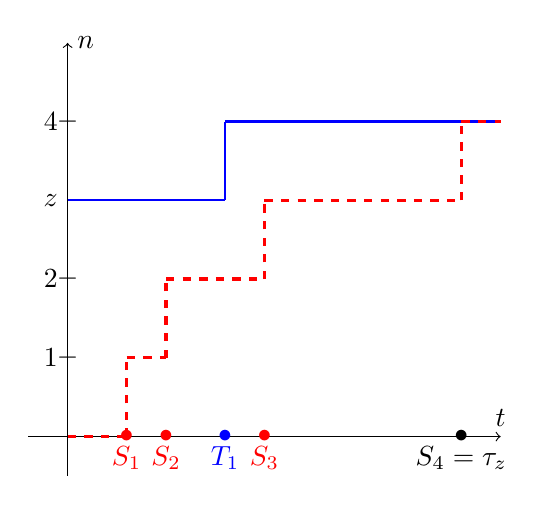
\begin{tikzpicture}
  %Origin and axis
  \coordinate (O) at (0,0);
  \draw[->] (-0.5,0) -- (5.5,0) coordinate[label = {above:$t$}] (xmax);
  \draw[->] (0,-0.5) -- (0,5) coordinate[label = {right:$n$}] (ymax);
 %Length of the honest chain
  \draw[thick,blue,-] (0,3) -- (2,3) node[pos=0.5, above] {} ;
  \draw[thick,blue] (2,3) -- (2,4) node[pos=0.5, above] {};
  \draw[thick,blue] (2,4) -- (5.5,4) node[pos=0.5, right] {};
  % %Length of the Malicious chain
  \draw[very thick,dashed,red,-] (0,0) -- (0.75,0) node[pos=0.5, above] {} ;
  \draw[very thick,dashed,red] (0.75,0) -- (0.75,1) node[pos=0.5, right] {};
  \draw[very thick,dashed,red] (0.75,1) -- (1.25,1) node[pos=0.5, above] {};
  \draw[very thick,dashed,red] (1.25,1) -- (1.25,2) node[pos=0.5, right] {};
  \draw[very thick,dashed,red] (1.25,2) -- (2.5,2) node[pos=0.5, above] {};
  \draw[very thick,dashed,red] (2.5,2) -- (2.5,3) node[pos=0.5, right] {};
  \draw[very thick,dashed,red] (2.5,3) -- (5,3) node[pos=0.5, right] {};
  \draw[very thick,dashed,red] (5,3) -- (5,4) node[pos=0.5, above] {};
  \draw[very thick,dashed,red] (5,4) -- (5.5,4) node[pos=0.5, above] {};
  %Jump Times of the malicious chain
  \draw (0.75,0) node[red,below] {$S_1$} node{ \color{red}$\bullet$};
  \draw (1.25,0) node[red,below] {$S_2$} node{ \color{red}$\bullet$};
  \draw (2.5,0) node[red,below] {$S_3$} node{ \color{red}$\bullet$};
  \draw (5,0) node[black,below] {$S_4=\tau_z$} node{ \color{black}$\bullet$};
  % %Jump Times of the honest chain
  \draw (2,0) node[blue,below] {$T_1$} node{ \color{blue}$\bullet$};
  % %Aggregated Capital gains
  \draw (0,1) node[black,left] {$1$} node{ \color{black}$-$};
  \draw (0,2) node[black,left] {$2$} node{ \color{black}$-$};
  \draw (0,3) node[black,left] {$z$} node{};
  \draw (0,4) node[black,left] {$4$} node{ \color{black}$-$};
  % %Ruin time = First-meeting time
  % \draw (7,0) node[black,below] {$\tau_z$} node{ \color{black}$\times$};
  % \draw[dotted,black] (7,3) -- (7,0);
\end{tikzpicture}
\end{center}
\caption{Illustration of the double spending problem within a continuous time framework.}
\label{fig:ds_poisson_process_illustrated}
\end{figure}
The double spending probability is given by the following result
\begin{theo}\label{theo:ds_probability_Poisson_process}
The double spending probability is given by 
$$
\mathbb{P}(\tau_z < \infty) = \left(\frac{\mu}{\lambda}\right)^z.
$$
\end{theo}
\begin{proof}
We make an analogy with \cref{sssec:insurance_risk_theory}, where $z$ is the inital reserves, $N_t$ is the premium income and $M_t$ is the liability of an insurance company. Define the claim surplus process as 
$$
S_t = M_t - N_t,\text{ }t\geq0.
$$
Note that $(S_t)_{t\geq0}$ is a L\'evy process such that $S_t\rightarrow + \infty$ beacuse $\lambda >\mu$. The equation 
$$
\kappa(s) =\log\mathbb{E}\left(e^{s S_1}\right) = 0
$$
is equivalent to 
$$
\mu \e^s + \lambda \e^{-s}- (\mu+\lambda) =0,
$$
which has a unique non negative solution given by 
$$
\gamma = \log\left(\frac{\lambda}{\mu}\right).
$$
It follows from \cref{prop:wald_martingale_levy} that $(\e^{\gamma S_t})_{t\geq 0}$ is a martingale, and applying \cref{prop:ruin_proba_levy} yields the double spending probability 
$$
\mathbb{P}(\tau_z<\infty) = \left(\frac{\mu}{\lambda}\right)^z,
$$
since $\xi(z)=0$ as ruin occurs exactly.
\end{proof}
\subsubsection{Double spending time}\label{sssec:double_spending_counting_process_dst}
Just like in \cref{sssec:double_spending_rw_dst}, we are interested in the time required to complete a double spending attack. Accounting for the cost of electricity, we can approximate the operational cost per time unit by 
$$
c = \pi_W\cdot W\cdot q,
$$
where 
\begin{itemize}
  \item $\pi_W$ is the electricity cost
  \item $W$ is the electricity consumed by the network
  \item  $q$ is the attacker's hashpower
\end{itemize}
The double spending cost reduces to $\tau_z\cdot c$. the following result provides a formula for the \pdf of $\tau_z$.
\begin{theo}
If $(N_t)_{t\geq0}$ is a Poisson process and $(M_t)_{t\geq0}$ is a renewal process then the \textbf{p.d.f.} of $\tau_z$ is given by
\begin{equation}\label{eq:DS_time_pdf}
f_{\tau_z}(t)=\mathbb{E}\left[\frac{z}{z+N_t}f_{S_{N_t+z}}(t)\right],\text{ for }t\geq0.
\end{equation}
\end{theo}
\begin{proof}
The event $\{\tau_z\in(t,t+\text{d}t)\}$, for $t\geq0$, corresponds to the exact time at which the double-spending attack is successful as the malicious chain takes over the honest one. At time $t=0$, the honest chain is ahead by $z\geq 1$ blocks. Assuming that later, at time $t>0$, the honest miners manage to add $N_t=n\in\mathbb{N}$ blocks to the chain then the malicious chain must be of length $M(t^{-})=n+z-1$ at some time $t^{-}<t$ and jumps to the level $n+z$ exactly at $t$. Conditioning over the values of $\{N_t\text{ , }t\geq0\}$ yields
\begin{equation}\label{eq:Tauz}
\{\tau_z\in(t,t+\text{d}t)\}=\bigcup_{n=0}^{+\infty}\{\tau_z\in(t,t+\text{d}t)\}\cap\{N_t=n\}.
\end{equation}
In the case where $N_t=0$, the only requirement is that the $z^{\text{th}}$ jump of $(M_t)_{t\geq0}$ occurs at time $t$. It then follows that
\begin{equation}\label{eq:TauzNt0}
\{\tau_z\in(t,t+\text{d}t)\}\cap\{N_t=0\}=\{S_{z}\in(t,t+\text{d}t)\}\cap\{N_t=0\},
\end{equation}
and consequently
\begin{equation}\label{eq:PDFTauzNt0}
f_{\tau_z|N_t}(t|0)=f_{S_z}(t),\text{ }t\geq0,
\end{equation}
where $f_{\tau_z|N_t}(t|0)$ denotes the conditional \pdf of $\tau_z$ given that $N_t=0$. On the set $\{N_t\geq1\}$, one needs to make sure that $\{M_t\text{ , }t\geq0\}$ behaves properly by constraining its jump times so that it does not reach $N_s+z$ at any time $s<t$ and performs the $(n+z)^{\text{th}}$ jump at $t$. Hence, it holds that
\begin{equation*}
\{\tau_z\in(t,t+\text{d}t)\}\cap\{N_t\geq1\}=\bigcup_{n=1}^{+\infty}\bigcap_{k=1}^{n}\{T_k\leq S_{z+k-1}\}\cap\{S_{z+n}\in(t,t+\text{d}t)\}\cap\{N_t=n\}.
\end{equation*}
Applying the law of total probability yields
\begin{eqnarray}
&&\mathbb{P}\left(\{\tau_z\in(t,t+\text{d}t)\}\cap\{N(t)\geq1\}\right)\nonumber\\
&=&\sum_{n=1}^{+\infty}\mathbb{P}\left[\bigcap_{k=1}^{n}\{T_k\leq S_{z+k-1}\}\cap\{S_{z+n}\in(t,t+\text{d}t)\}\Big\rvert N(t)=n\right]\mathbb{P}[N(t)=n].\label{eq:LawOfTotalProbabilityTh1}
\end{eqnarray}
In virtue of the order statistic property, the successive jump times $(T_1,\ldots,T_n)$ are distributed as the order statistics $(V_{1:n},\ldots,V_{n:n})$ of a sample of $n$ \iid random variables uniformly distributed on $(0,t)$. The conditional probability in \eqref{eq:LawOfTotalProbabilityTh1} may be rewritten as
\begin{eqnarray}
&&\mathbb{P}\left[\bigcap_{k=1}^{n}\{V_{k:n}\leq S_{z+k-1}\}\cap\{S_{z+n}\in(t,t+\text{d}t)\}\right]\nonumber\\
&=&\mathbb{P}\left[\bigcap_{k=1}^{n}\{U_{k:n}\leq S_{z+k-1}/ t\}\cap\{S_{z+n}\in(t,t+\text{d}t)\}\right]\nonumber\\
&=&\mathbb{P}\left[\bigcap_{k=1}^{n}\{U_{k:n}\leq S_{z+k-1}/t\}\big\rvert S_{z+n}\in(t,t+\text{d}t)\right]\mathbb{P}[S_{z+n}\in(t,t+\text{d}t)]\nonumber\\
&=&\mathbb{E}\left\{(-1)^{n}G_{n}[0\big\rvert S_{z}/t,\ldots, S_{z+n-1} / t] \big\rvert S_{z+n}\in(t,t+\text{d}t)\right\}\mathbb{P}[S_{z+n}\in(t,t+\text{d}t)],\nonumber\\
&=&(-1/t)^{n}\mathbb{E}\left\{G_{n}[0\big\rvert S_{z},\ldots, S_{z+n-1}] \big\rvert S_{z+n}\in(t,t+\text{d}t)\right\}\mathbb{P}[S_{z+n}\in(t,t+\text{d}t)],\nonumber\\
&&\label{eq:AGPolynomialsProof}
\end{eqnarray}
where $U_{1:n},\ldots,U_{n:n}$ denote the order statistics of a sample of $n$ \iid uniform random variables on $(0,1)$, and $G_n(.|.)$ correspond to the sequence of A-G polynomials as defined in \cref{sssec:exp_distribution}. The last equation in \eqref{eq:AGPolynomialsProof} follows from using the first identity of \cref{prop:Appell_AG_polynomials_properties}.
Inserting \eqref{eq:AGPolynomialsProof} into \eqref{eq:LawOfTotalProbabilityTh1} and letting $\text{d}t$ be small enough yields
\begin{eqnarray}
f_{\tau_z|N(t)\geq1}(t)&=&\sum_{n=1}^{+\infty}(-1/t)^{n}\mathbb{E}\left\{G_{n}[0\big\rvert S_{z},\ldots,S_{z+n-1}] \big\rvert S_{z+n}=t\right\}\nonumber\\
&\times&f_{S_{z+n}}(t)\mathbb{P}[N(t)=n]\label{eq:cond_pdf_tau_N_greater_than_1}.
\end{eqnarray}
We further work on the AG polynomials to simplify the above expressions. We have that
\begin{eqnarray} 
\mathbb{E}\left\{G_{n}(0\big\rvert S_{z},\ldots,S_{z+n-1}) \rvert S_{z+n}=t\right\}&=& \mathbb{E}\left\{G_{n}(-S_z\rvert 0,\ldots,S_{z+n-1}-S_z) \rvert S_{z+n}=t\right\} \nonumber\\
&=& \mathbb{E}\left\{\mathbb{E}\left[G_{n}(-S_z\rvert 0,\ldots,S_{z+n-1}-S_z)\rvert S_{z+n}-S_z, S_{z+n}\right] \rvert S_{z+n}=t\right\} \nonumber\\
&=& \mathbb{E}\left\{(-S_z)(-S_z-S_{n+z}+S_z)^{n-1} \rvert S_{z+n}=t\right\} \nonumber\\
&=& (-1)^n\mathbb{E}\left\{S_z S_{n+z}^{n-1} \rvert S_{z+n}=t\right\} \nonumber\\
&=& (-1)^nt^{n-1}\frac{z}{z+n}t =(-t)^n\frac{z}{z+n} \label{eq:AG_polynomial_simplification}
\end{eqnarray}
Inserting \eqref{eq:AG_polynomial_simplification} into \eqref{eq:cond_pdf_tau_N_greater_than_1} yields
\begin{equation*}
f_{\tau_z|N_t\geq1}(t)=\sum_{n=1}^{+\infty}\frac{z}{z+n}f_{S_{z+n}}(t)\mathbb{P}(N_t=n)
\end{equation*}
The final step consists in adding the case $N_t=0$ to the sum, therefore writing
\begin{equation*}
f_{\tau_z}(t)=\sum_{n=0}^{+\infty}\frac{z}{z+n}f_{S_{z+n}}(t)\mathbb{P}(N_t=n)
\end{equation*}
which is equivalent to the announced result \eqref{eq:DS_time_pdf}.  
\end{proof}
\begin{remark}
Just like in the random walk framework of \cref{ssec:double_spending_rw}, the number $z$ is actually a random variable defined as 
$$
Z = (\alpha - M_{T_\alpha})_+,
$$
where $T_\alpha$ is the arrival time of the $\alpha^{th}$ block in the main branch of the blockchain. If $(M_t)_{t\geq0}$ is a Poisson process with intensity $\mu$ then $M_{T_\alpha})$ is mixed Poisson distributed with parameter $\mu\cdot T_{\alpha}$. We have that 
\begin{eqnarray*}
\mathbb{P}(M_{T_\alpha} = m) &=& \int_{0}^{\infty}\frac{\e^{-\mu t}(\mu t)^m}{m!}\frac{\e^{-\lambda t}t^{\alpha-1}\lambda ^\alpha}{(\alpha -1)}\text{d}t\\
&=&\frac{\mu^m\lambda^{\alpha}}{m!(\alpha-1)!}\int_{0}^{\infty}\e^{-t(\mu + \lambda)}t^{m+\alpha-1}\text{d}t\\
&=&\binom{m+\alpha-1}{m}\left(\frac{\lambda}{\lambda+\mu}\right)^{\alpha}\left(\frac{\mu}{\lambda+\mu}\right)^{m}.
\end{eqnarray*}
The number of blocks found by the attacker until the vendor's transaction gets $\alpha$ confirmations is governed by a negative binomial distribution.
\end{remark}
\section{Blockwitholding in PoW}\label{sec:blockwithholding}
Blockwitholding is a deviation from the prescribed protocol in which miner would constitute a stock of block to be released aat well chosen time in order to fork the chain. We focus in this section on the first blockwitholding strategy called selfish mining and described in \citet{Eyal2014}.
\subsection{The selfish mining strategy}\label{ssec:selfish_mining}
\subsection{Ruin and expected profit of a miner}\label{ssec:selfish_mining}
\subsection{Ruin and expected profit of a selfish miner}\label{ssec:selfish_mining}

\section{Nothing-at-stake in PoS}\label{sec:NaS}
\newpage